\section{Evaluation}
\label{sec:evaluation}
If not differently specified, all experiments discussed in this section are run with the following parameters: $N = 500$, $n_{max} = 200$, $n_D = 100$ and $c = 0$.

\subsection{Storage Capacity}
\label{subsec:capacity}
\begin{figure}[t]
	\centering
	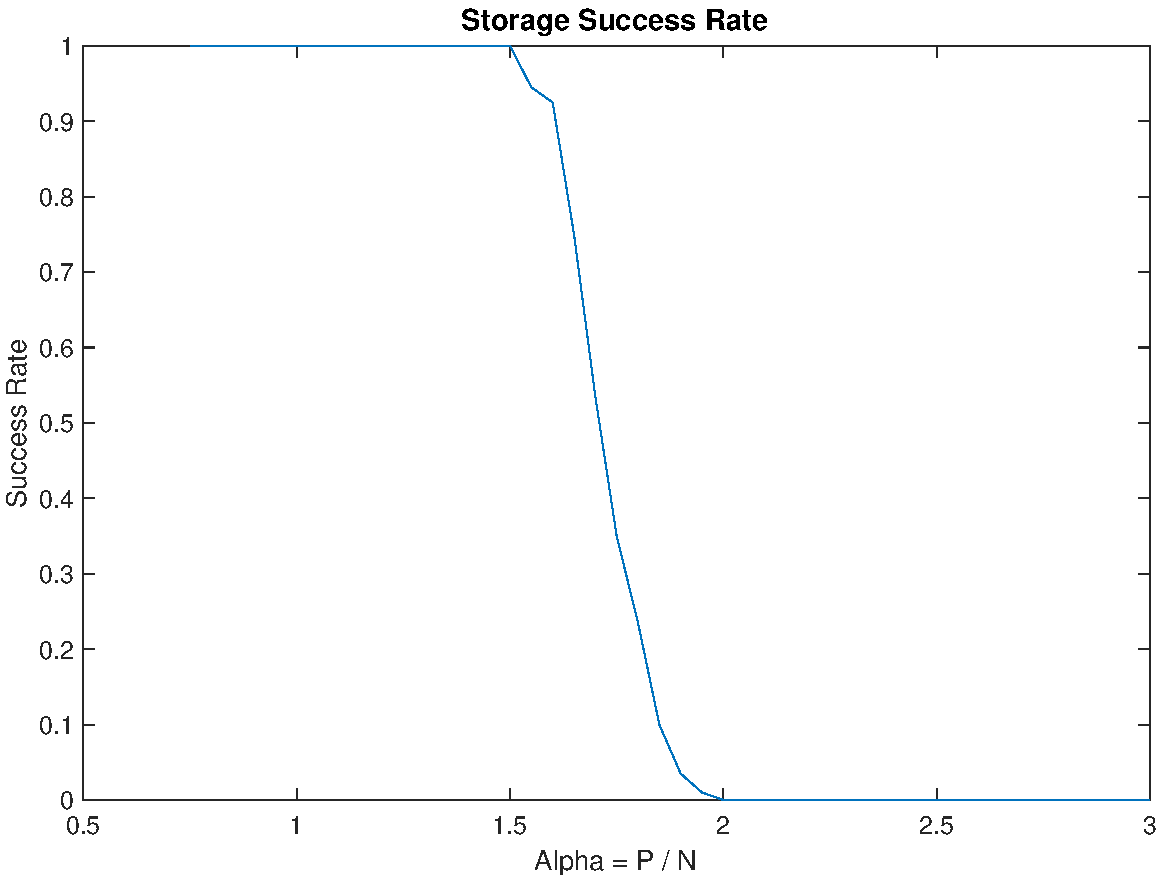
\includegraphics[width=\columnwidth]{figures/base}
    \caption{Storage success rate of a Rosenblatt perceptron as a function of $\alpha = P / N$. The experiments use $N = 500$, $n_{max} = 200$ and $n_D = 100$.}
	\label{fig:base}
\end{figure}
\cref{fig:base} shows the results of the base experiment.
The x-axis represent different values of $\alpha = P / N$, while the y-axis the success rate $Q_{l.s.}$.
As expected, the function looks like a step function from $1$ to $0$.
For $\alpha \approx 1.7$, the success rate $Q_{l.s.}$ drops from $1$ to $0$ very quickly. 

The value of $\alpha$ for which the function drops is called storage capacity of the perceptron.
For $N \to \infty$ (very large number of examples) and $n_{max} \to \infty$ (no limit on the maximum number of training iterations), the theoretical storage capacity of the Rosenblatt perceptron is $\alpha = 2$.

\subsection{Number of Iterations}
\label{subsec:epochs}
\begin{figure}[t]
	\centering
	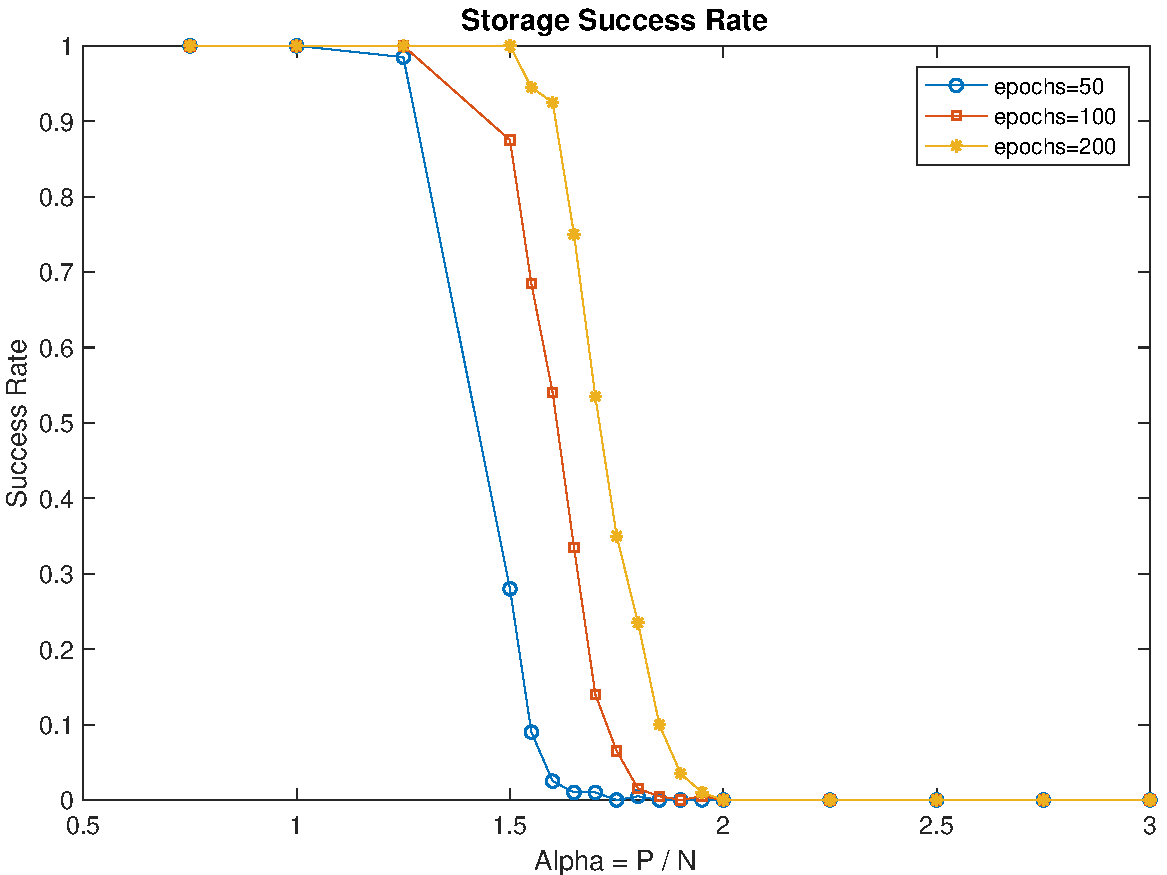
\includegraphics[width=\columnwidth]{figures/multiple_epochs}
    \caption{Storage success rate of a Rosenblatt perceptron as a function of $\alpha = P / N$ for different values of $n_{max}$.}
	\label{fig:multiple_epochs}
\end{figure}

The difference between the theoretical value and the experimental one are mainly due to the limited number of training iterations.
\cref{fig:multiple_epochs} gives an experimental proof of this statement:
for a very small number of iterations (eg. $n_{max} = 10$), the step is close to $\alpha = 1$, while for higher values of iterations the step moves closer and closer to the theoretical value $\alpha = 2$ found with \cref{eq:prob-lin-sep-alpha}.
The theoretical result still remains far from the practical one because of the limited size of input's dimension $N$.

\subsection{Number of Dimensions}
\label{subsec:dimensions}
\begin{figure}[t]
	\centering
	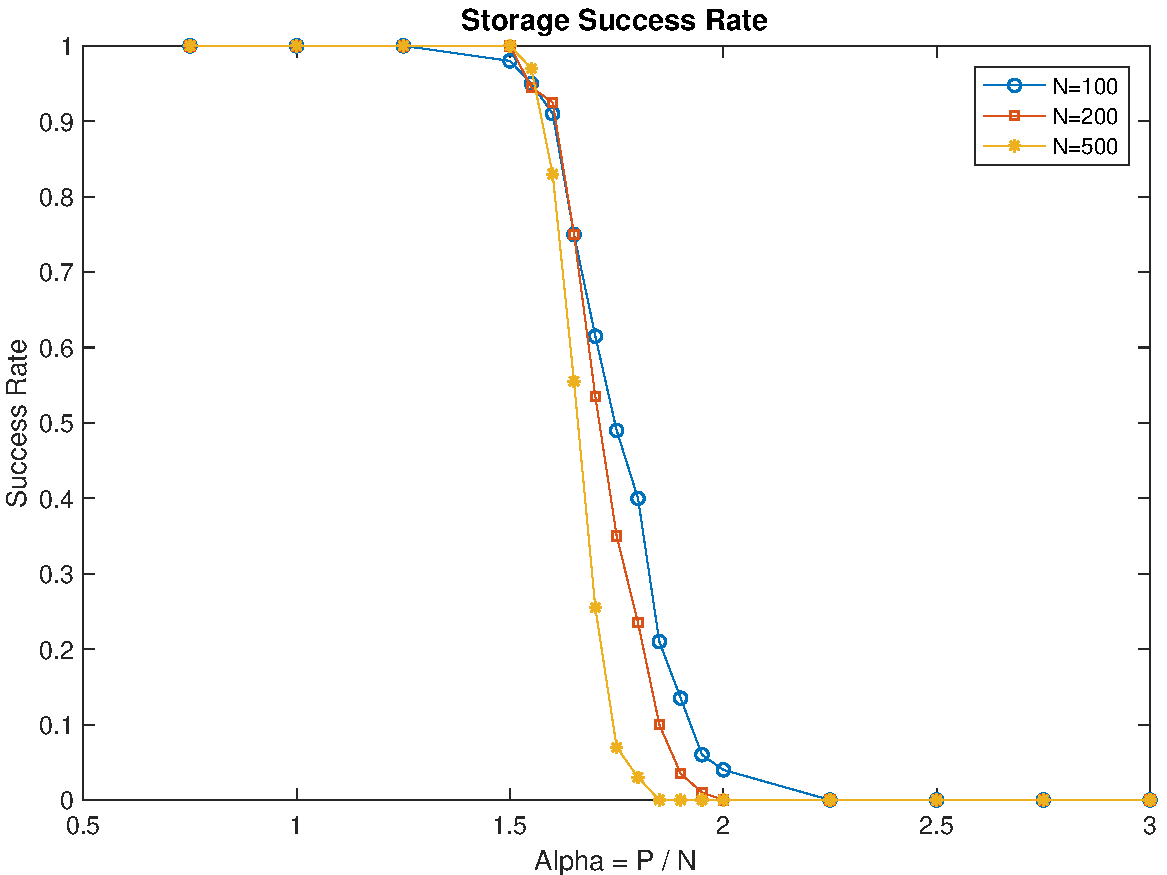
\includegraphics[width=\columnwidth]{figures/multiple_n}
    \caption{Storage success rate of a Rosenblatt perceptron as a function of $\alpha = P / N$ for different values of $N$.}
	\label{fig:multiple_n}
\end{figure}
The theoretical results are valid for $N \to \infty$.
However, real datasets have a limited number of features.
\cref{fig:multiple_n} shows the behaviour of the perceptron for different values of $N$.
For high values of $N$, the shape of the success rate $Q_{l.s.}$ as a function of $\alpha$ is similar to a step function.
For small values of $N$, the function looks like a smoothed step function:
the smaller $N$ is, the higher is the smoothing.

\subsection{Weight Update Criterion}
\label{subsec:c}
\begin{figure}[t]
	\centering
	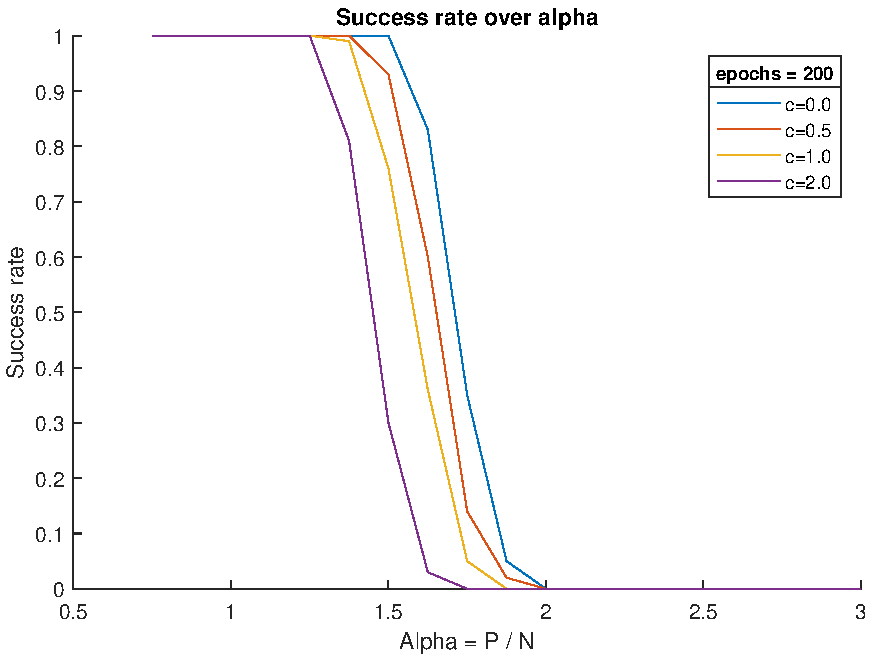
\includegraphics[width=\columnwidth]{figures/bonus_2_c}
    \caption{Storage success rate of a Rosenblatt perceptron as a function of $\alpha = P / N$ for different values of $c$.}
	\label{fig:multiple_c}
\end{figure}
\cref{fig:multiple_c} shows the effect of changing the values of $c$ in the training procedure for the perceptron.
For higher values of $c$, the curve is shifted to the left.
Since an example $\xi^\mu$ is considered correctly classified only when its local potential is greater then $c$ ($E = \mathsf{\bm{w}} \cdot \xi^\mu S^\mu > c$), the potential only depends on $\mathsf{\bm{w}}$ for a fixed $\xi^\mu$ and the update of $\mathsf{\bm{w}}$ is fixed for a given wrong classified example, the perceptron will need a higher number of updates to increase the norm of $\mathsf{\bm{w}}$ and make the local potentials higher then a threshold $c > 0$.
Formally, we can show that the value of $c > 0$ is irrelevant (provided the perceptron is trained long enough):
\begin{equation*}
	\mathsf{\bm{w}}_1 : \{E_1^\mu \geq c\}_{\mu = 1}^{P} \Leftrightarrow \mathsf{\bm{w}}_2 = \lambda \mathsf{\bm{w}}_1 : \{E_2^\mu \geq c\}_{\mu = 1}^{P}, \lambda > 0
\end{equation*}

\begin{figure}[t]
	\centering
	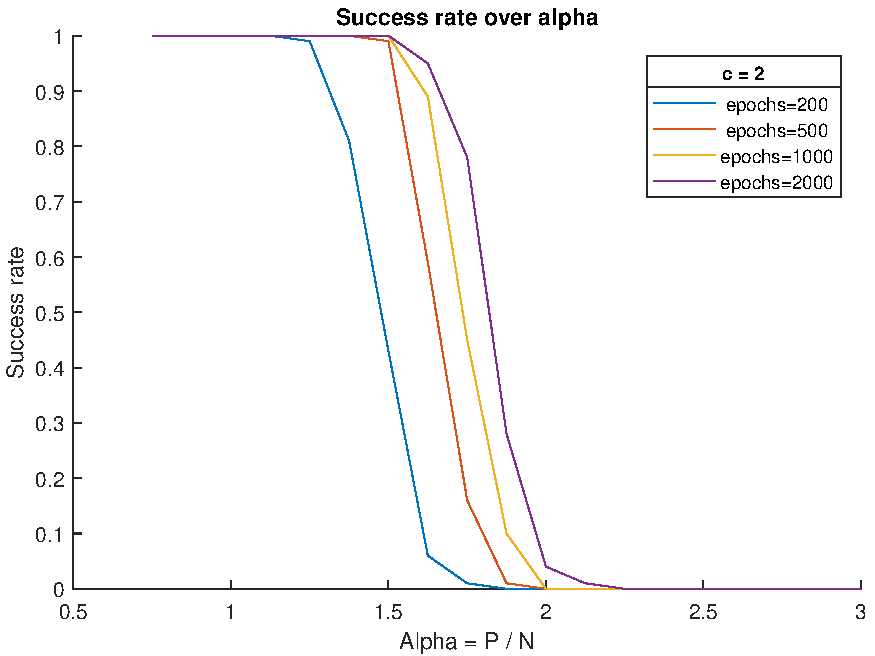
\includegraphics[width=\columnwidth]{figures/bonus_2_epoch}
    \caption{Storage success rate of a Rosenblatt perceptron as a function of $\alpha = P / N$ for different numbers of iterations with fixed value of $c=2$.}
	\label{fig:fixed_c_multiple_epoch}
\end{figure}
To give an empirical proof of this, we fix the value of $c$ and train the perceptron for different number of iterations $n_{max}$.
We expect to see the curve shifted to the left for small $n_{max}$, and approximate a step function centered in $\alpha = 2$ for big $n_{max}$.
\cref{fig:fixed_c_multiple_epoch} shows that the results of the experiment confirm our hypothesis.

\begin{figure}[t]
	\centering
	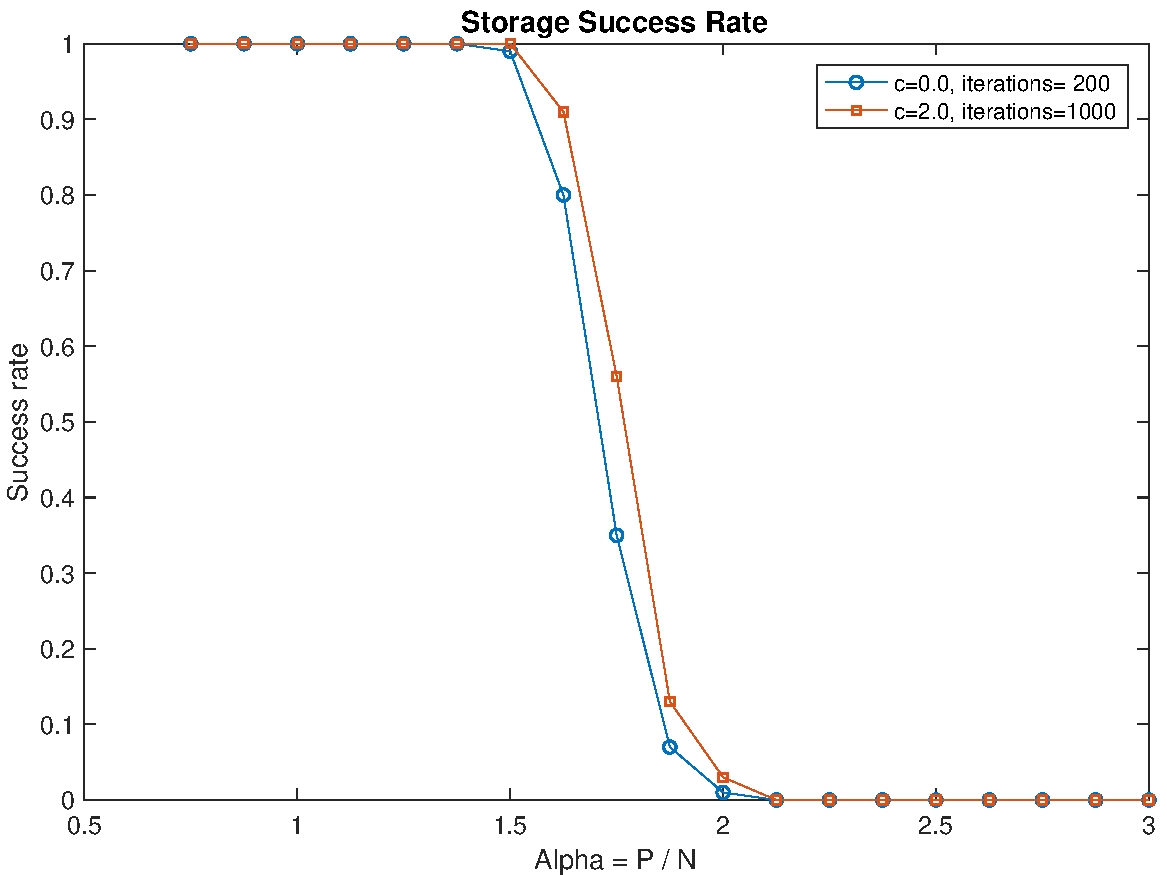
\includegraphics[width=\columnwidth]{figures/bonus_2_c_epoch}
    \caption{Storage success rate of a Rosenblatt perceptron as a function of $\alpha = P / N$ for different numbers of iterations and $c$.}
	\label{fig:multiple_c_multiple_epoch}
\end{figure}
\cref{fig:multiple_c_multiple_epoch} compares the curves for $c = 0$ and $c = 2.0$ for different values of $n_{max}$:
by increasing $n_{max}$, the curve is ``pushed'' towards the right, contrasting the effect of the increased value of $c$.
We can somehow see $c$ as a simple version of the learning rate that is used in more complex neural networks: it ``regulates'' the speed of the training.

\subsection{Inhomogeneous Hyperplanes}
\label{subsec:homogeneous}
\begin{figure}[t]
	\centering
	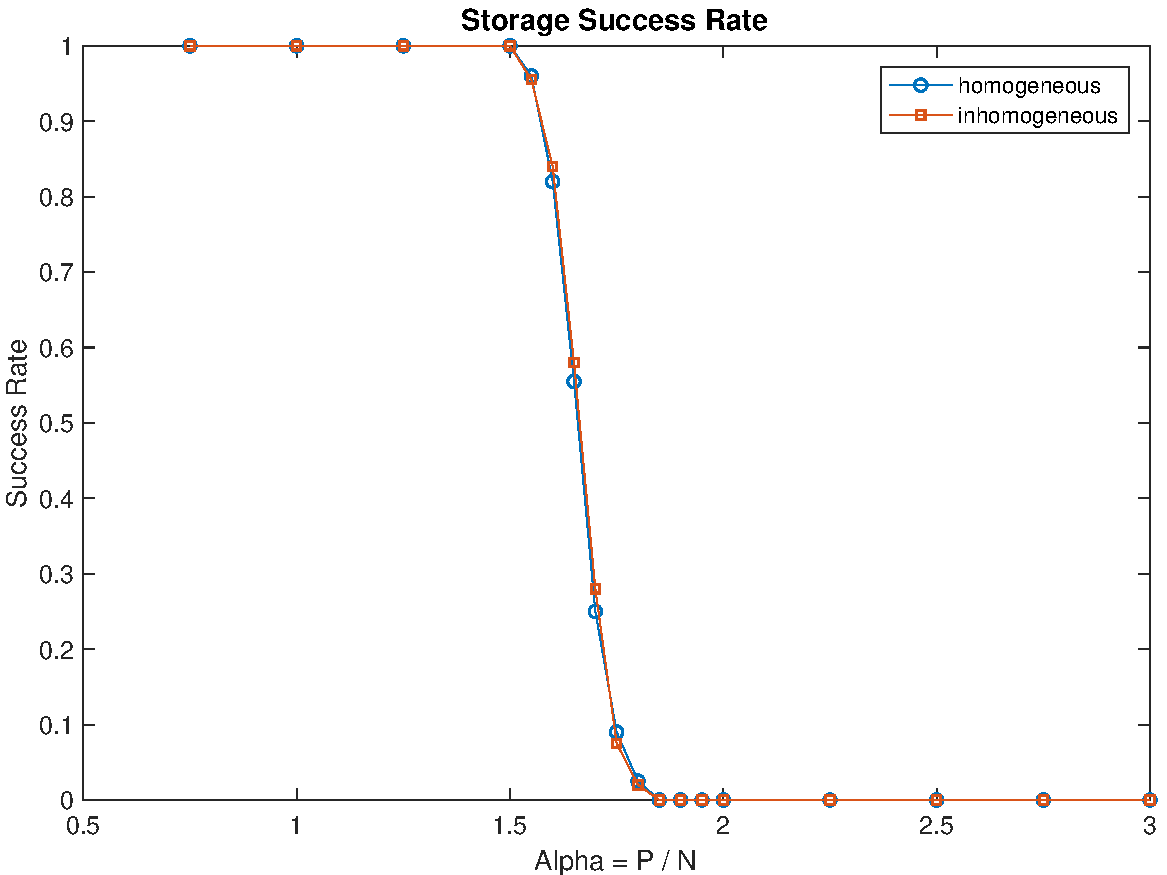
\includegraphics[width=\columnwidth]{figures/homogeneous}
    \caption{Storage success rate of a Rosenblatt perceptron and its inhomogeneous version for $N = 500$ as a function of $\alpha = P / N$.}
	\label{fig:homogeneous}
\end{figure}
We run an experiment to verify the behaviour of $Q_{l.s.}$ by allowing inhomogeneous hyperplanes:
we train both a normal and modified perceptron on $200$ different datasets using $N = 500$, $n_{max} = 200$.
\cref{fig:homogeneous} shows the results of the experiment.
As expected, the success rate $Q_{l.s.}$ of the inhomogeneous perceptron is slightly higher than homogeneous one.
However, the difference is not significant, since data points follow a normal distribution $\xi^\mu_j \sim \mathcal{N}(0,\,1)$ and are therefore distributed around the origin.

The problem of finding an inhomogeneously solution in $R^{N}$ can be solved by finding a homogeneously solution in $R^{N + 1}$.
In a second experiment, we compare the success rate $Q_{l.s.}$ of an inhomogeneous perceptron for $N = 500$ with an homogeneous perceptron for $N = 501$.
\cref{fig:homogeneous_n_n1} shows the result of this experiment.
As expected, the success rates for the $2$ perceptrons are very close to each other.

\begin{figure}[t]
	\centering
	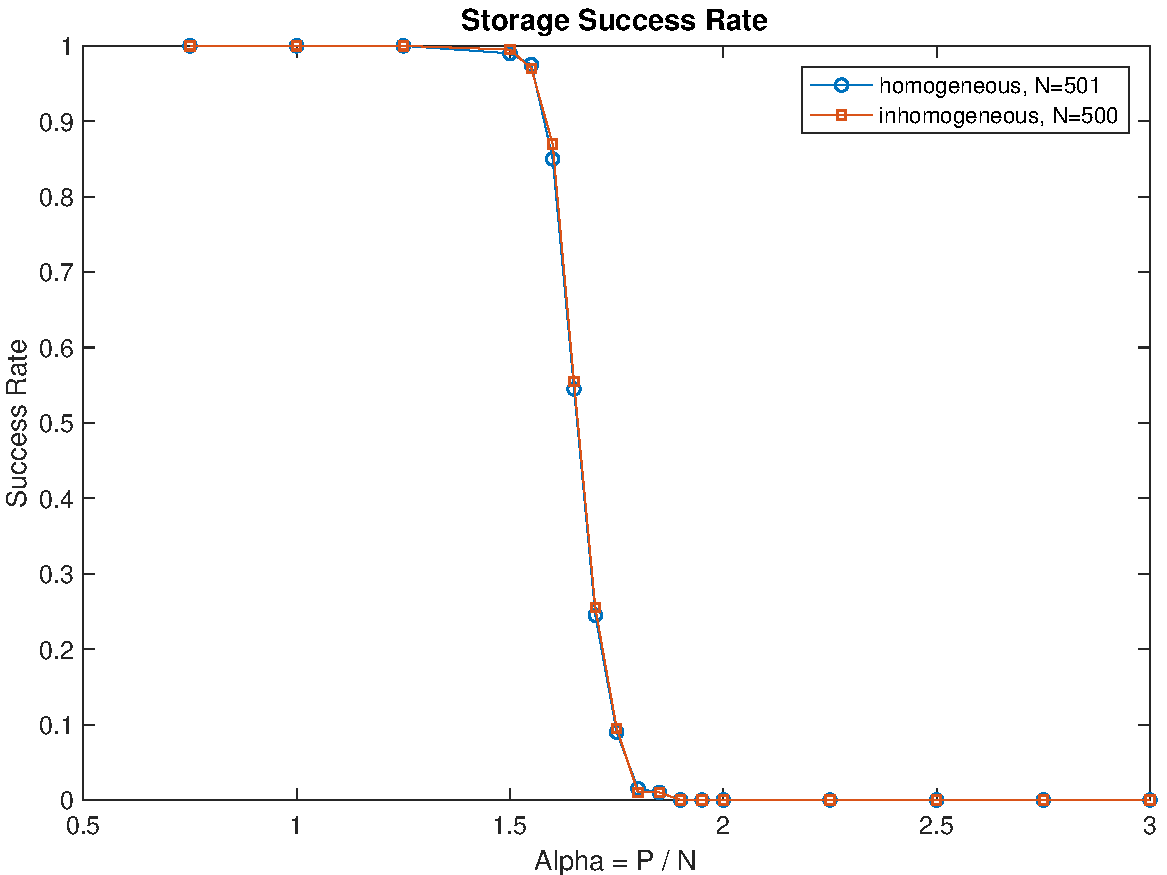
\includegraphics[width=\columnwidth]{figures/homogeneous_n_n1}
    \caption{Storage success rate of a homogeneous Rosenblatt perceptron for $N = 501$ and its inhomogeneous version for $N = 500$ as a function of $\alpha = P / N$.}
	\label{fig:homogeneous_n_n1}
\end{figure}
